\documentclass{main.tex}[subfiles]
\begin{document}
\section{Метод полуконтролируемого обучения с автоматическим исправлением ошибок}
\subsection{Предварительная обработка текста}
\subsection{Построение выравнивания}
Будем называть \emph{референсом (reference)} исходный текст и \emph{запросом (query)} строку, полученную в результате распознавания страницы (эти термины используются в биоинформатике, в задаче нахождения сходства между биологическими последовательностями).
Пусть эти две строки содержат только символы из некоторого алфавита $\mathcal A $. Введём символ \emph{пробела}: $ \ast \notin \mathcal A $.

\emph{Выравниванием} будем называть две строки одинаковой длины, полученные из референса и запроса вставкой нужного количества символов $\ast$ на некоторых позициях.
Выравнивание задаёт соответствие между символами двух строк с одинаковыми индексами (говорят, что символ из одной строки \emph{выравнивается} на другой); цель -- поиск наилучшего соответствия, содержащего как можно меньше пропусков и как можно больше попарных совпадений символов.

Ситуацию, когда два соответствующих символа в выравнивании различные и оба не являются пропусками, называют \emph{несовпадением (mismatch)}.
Если символ референса выравнивается на пропуск, это называют \emph{выпадением (deletion)}; выравнивание символа запроса на пробел -- \emph{вставка (insertion)}.
В нашей задаче, построив выравнивание, можно скорректировать метку класса в случае несовпадения или удалить метку в случае вставки.
Найденные выпадения никак не исправляются, поскольку мы не знаем, в каком месте изображения находится выпавший символ; в некоторых случаях можно попытаться определить место, где находится выпавшая буква, исходя из пространственного расположения соседних символов, но это выходит за рамки данной работы. \\

Похожие методы исправления символов ранее были разработаны для обычных программ распознавания текста по изображениям \cite{muller2021word_aln}.

\subsubsection{Поиск регионов интереса. Хэширование}
\subsubsection{Оптимальное выравнивание. Алгоритм Нидлмана-Вунша}

Нидлман и Вунш \cite{needleman1970} разработали алгоритм, который находит оптимальное выравнивание, т. е. то, которое содержит наименьшее возможное число несовпадений

\begin{verbatim}
    homo homini lupus est
    hom***o**ni lupus****
\end{verbatim}

Теорема. Алгоритм () % TODO
строит выравнивание с наименьшим возможным числом несовпадений на участке от первого отличного от пропуска символа запроса до последнего.


\begin{figure}[H]
    \centering
    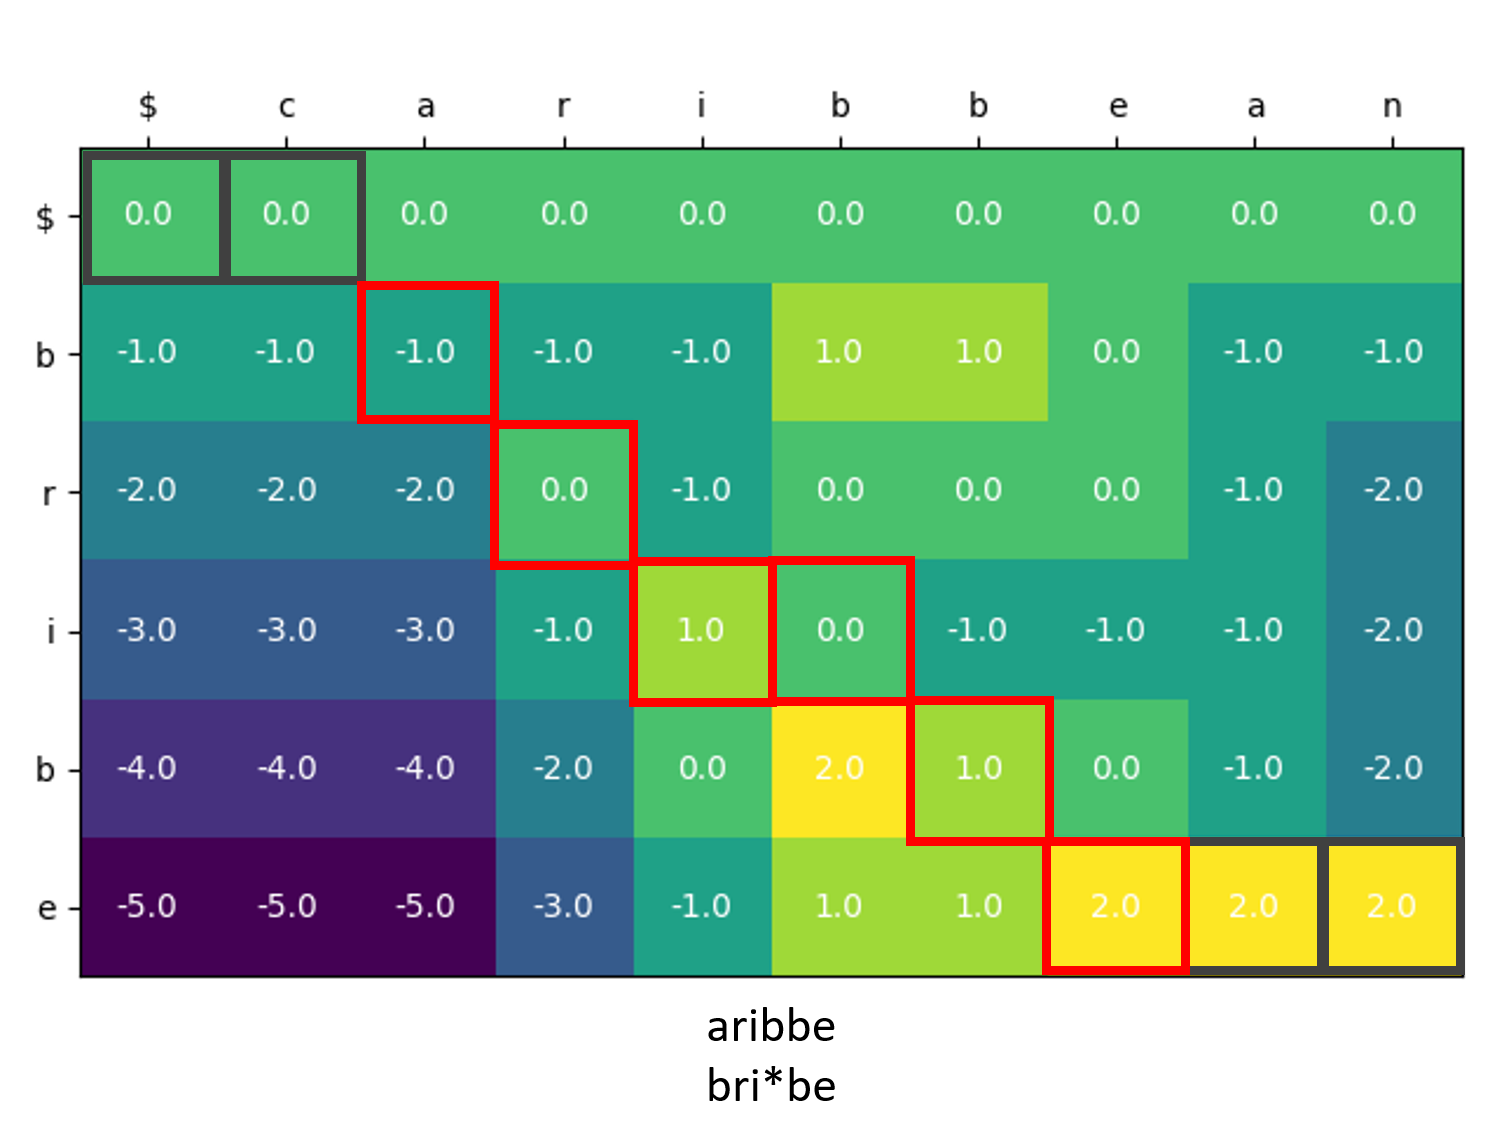
\includegraphics[width=\myPictWidth]{test_needleman_wunsch/caribbean_bribe}
    \caption{Матрица динамического программирования модифицированного алгоритма Нидлмана-Вунша для референса "caribbean"\hspace{0pt} и запроса "bribe". Жирными линиями обведены клетки, соотвтествующие найденному выравниванию }
    \label{fig:caribbean_bribe} % TODO ref in the text
\end{figure}

\begin{figure}[H]
    \centering
    \begin{subfigure}{.5\textwidth}
        \centering
        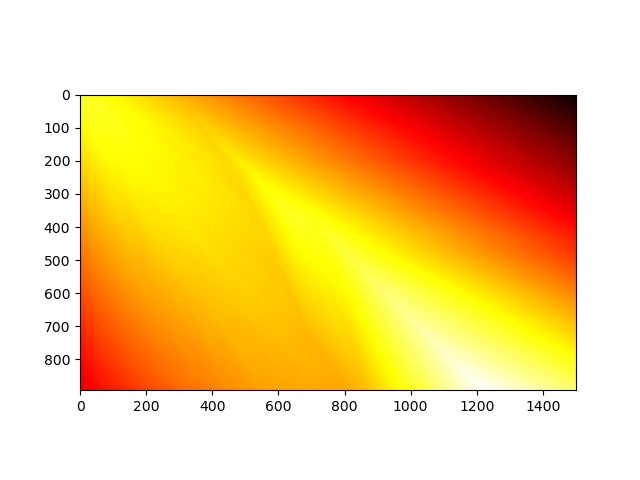
\includegraphics[width=\myPictWidth]{test_needleman_wunsch/big_penalizeTrue}
        \caption{обычный алгоритм}
        % TODO \label{fig:}
    \end{subfigure}%
    \begin{subfigure}{.5\textwidth}
        \centering
        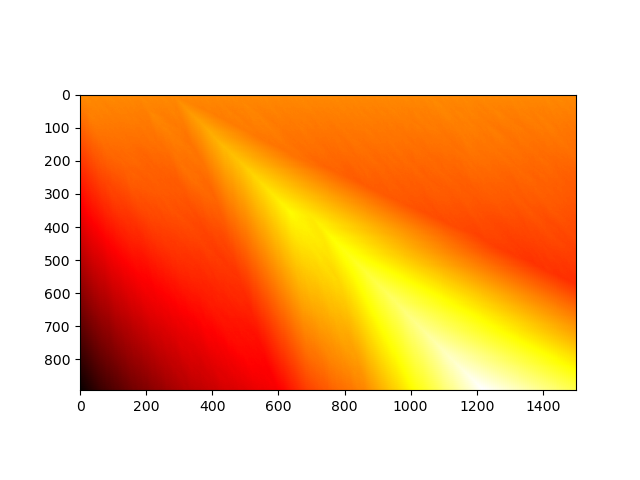
\includegraphics[width=\myPictWidth]{test_needleman_wunsch/big_penalizeFalse}
        \caption{модифицированный алгоритм}
        % TODO \label{fig:}
    \end{subfigure}
    \caption{Тепловые карты матриц динамического программирования при выравнивании результата распознавания страницы из романа "Scarlet Letter"\hspace{0pt} на участок, найденный с помощью хэширования на референсе.
    Более светлые точки сооветствуют элементам матрицы с более высоким значением.}
    \label{fig:needleman_real} % TODO ref in the text
\end{figure}

\subsection{Исправление ошибок после выравнивания}
\end{document}